%% start of file `template.tex'.
%% Copyright 2006-2013 Xavier Danaux (xdanaux@gmail.com).
%
% This work may be distributed and/or modified under the
% conditions of the LaTeX Project Public License version 1.3c,
% available at http://www.latex-project.org/lppl/.


\documentclass[11pt,a4paper]{moderncv}        % possible options include font size ('10pt', '11pt' and '12pt'), paper size ('a4paper', 'letterpaper', 'a5paper', 'legalpaper', 'executivepaper' and 'landscape') and font family ('sans' and 'roman')
% moderncv themes
%\usepackage{fontspec}
%\setmainfont{Latin Modern Roman}
\usepackage{fontawesome}
\moderncvstyle{oldstyle}                             % style options are 'casual' (default), 'classic', 'oldstyle' and 'banking'
\moderncvcolor{blue}                               % color options 'blue' (default), 'orange', 'green', 'red', 'purple', 'grey' and 'black'
%\renewcommand{\familydefault}{\sfdefault}         % to set the default font; use '\sfdefault' for the default sans serif font, '\rmdefault' for the default roman one, or any tex font name
%\nopagenumbers{}                                  % uncomment to suppress automatic page numbering for CVs longer than one page
\usepackage[scaled]{helvet}
%\usepackage[T1]{fontenc}
\renewcommand{\familydefault}{\sfdefault}
\fontfamily{phv}\selectfont 
\usepackage[ngerman]{datetime}
% character encoding
\usepackage[normalem]{ulem}
\usepackage{epstopdf}
%use \MARVfax
\usepackage{graphicx}
\usepackage{tikz}
\usepackage{ragged2e}
\usepackage{footmisc} 
\usepackage{changepage}
\usepackage[utf8]{inputenc}  
\usepackage[absolute,overlay]{textpos}      
\urlstyle{same}
               % if you are not using xelatex ou lualatex, replace by the encoding you are using
%\usepackage{CJKutf8}                              % if you need to use CJK to typeset your resume in Chinese, Japanese or Korean

% adjust the page margins
\usepackage{epstopdf}
\usepackage{pdfpages}
\usepackage{geometry}
\geometry{bottom=1.5cm,top=2cm,left=2cm,right=1.5cm}
	\definecolor{airforceblue}{rgb}{0.19, 0.55, 0.91}
%\setlength{\hintscolumnwidth}{3cm}                % if you want to change the width of the column with the dates
%\setlength{\makecvtitlenamewidth}{10cm}           % for the 'classic' style, if you want to force the width allocated to your name and avoid line breaks. be careful though, the length is normally calculated to avoid any overlap with your personal info; use this at your own typographical risks...

% personal data
\name{Weiran}{Zhang}
%\title{Curriculum Vit\ae{}}                               % optional, remove / comment the line if not wanted
\address{}{}{}% optional, remove / comment the line if not wanted; the "postcode city" and and "country" arguments can be omitted or provided empty
\phone[mobile]{+49~(0)~0511-12275069}                   % optional, remove / comment the line if not wanted
\email{} 
                              % optional, remove / comment the line if not wanted
%\photo[64pt][0.4pt]{picture}                       % optional, remove / comment the line if not wanted; '64pt' is the height the picture must be resized to, 0.4pt is the thickness of the frame around it (put it to 0pt for no frame) and 'picture' is the name of the picture file


% to show numerical labels in the bibliography (default is to show no labels); only useful if you make citations in your resume
%\makeatletter
%\renewcommand*{\bibliographyitemlabel}{\@biblabel{\arabic{enumiv}}}
%\makeatother
%\renewcommand*{\bibliographyitemlabel}{[\arabic{enumiv}]}% CONSIDER REPLACING THE ABOVE BY THIS

% bibliography with mutiple entries
%\usepackage{multibib}
%\newcites{book,misc}{{Books},{Others}}
%----------------------------------------------------------------------------------
%            content
%----------------------------------------------------------------------------------
%some shadow

\begin{document}



%\clearpage%\end{CJK*}                              % if you are typesetting your resume in Chinese using CJK; the \clearpage is required for fancyhdr to work correctly with CJK, though it kills the page numbering by making \lastpage undefined

%%\newdateformat{myformat}{\THEDAY{ten }\monthname[\THEMONTH], \THEYEAR}
%\renewcommand{\familydefault}{\sfdefault}
\label{sec:Anschreiben}
\begin{minipage}[t][2cm][t]{0.6\linewidth}
	%\vspace{1cm}
	\normalfont
Dr. Fahland \\[0.5em]
Bundesanstalt für Geowissenschaften und Rohstoffe (BGR)\\
Geozentrum Hannover\\
Stilleweg 2\\
30655 Hannover\\
%(bevorzugter Einsatzort: Braunschweig)
%Büro Braunschweig
	\vfill
\end{minipage}
\hfill
\begin{minipage}[t][4.5cm][t]{0.3\linewidth}
	\raggedleft
	\small{ \color{darkgray}
		Absender:\\\vspace{0.5em}Weiran Zhang\\ \vspace{0.5em}
		Vincent-van-Gogh-Ring 3D\\ 38126 Braunschweig\\\vspace{0.5em}
		weiran-zhang@outlook.com\\
		+49~(0)176 2136 5452\\}
	\vspace{0.5em}
Stellenausschreibung: B 112/20\\[0.5em]
 \today
	\vfill	
\end{minipage}
\begin{minipage}[t][1cm][t]{1\linewidth}
	\large\textbf{Bewerbung als wissenschaftlicher Mitarbeiter (B 112/20)\\[1em]}
	%% "Gekoppelte	Modellberechnungen Endlagerung"
\end{minipage}

\begin{adjustwidth}{0cm}{1cm}
	Sehr geehrte Frau Dr. Fahland,\\[1em]
	 zuerst möchte ich mich bei Ihnen  für das freundliche Auswahlgespräch am 01.10.2020 bedanken. Ich habe weiterhin ein großes Interesse an der Forschung für langzeitsichere Endlagerung radioaktiver Abfälle, da dies ein entscheidendes Thema für eine sichere Zukunft ist. %Besonders hat das Mitteilungsschreiben von der Personalabteilung  mich beeindruckt, dass die BGR für jede Bewerbung sehr verantwortlich ist. Auch bin ich mir davon bewusst, dass meine Kenntnisse über thermo-hydro-mechanisch (THM) gekoppelte Prozessen noch verbessert werden soll.
	 Die Vielfältigkeit des Themas und dessen Anwendungsbereich motivieren mich meine Kenntnisse über thermo-hydro-mechanisch (THM) gekoppelte Prozessen zu verbessern und erweitern.\\[1em]
	  Vor einigen Tagen habe ich die mündliche Prüfung für meine Dissertation "Stochastische Modellierung und numerische Simulation von Ermüdungsschädigung" an der Leibniz Universität Hannover (LUH) abgeschlossen. Momentan bin ich auch auf der Suche nach neuen Forschungsstellen und bin dadurch auf Ihre Stellenausschreibung gestoßen, welche sich sehr gut mit meinem Interessengebiet im Bereich der Forschung deckt. %  Forschung zu treiben und anwendungsorientiert zu arbeiten, bin ich auf diese Stellenausschreibung gestoßen. %Die Stellenausschreibung motiviert mich, eine erneute Bewerbung bei Ihnen einzureichen. 
	 % Mein Plan für die Postdoc-Phase ist mit der Fachkollegen jedes Jahr neue Veröffentlichungen zu haben, damit meine Berufsentwicklung in der Akademie nachvollziehbar ist. Die Aufgaben der Stelle haben einigen Zusammenhang mit meinen bisherigen Erfahrungen, als Beispiele:\\[-0.5em]
	 Ich konnte einige Zusammenhänge zwischen den beschriebenen Aufgaben und meinen bisherigen Erfahrungen finden und möchte Ihnen diese  erläutern:\\[-0.5em]
		\begin{adjustwidth}{0.5cm}{0cm}
					\begin{itemize}	
	\item[$\bullet$] Das Kluftnetz und die Schichtungen des porösen Mediums könnte durch einen Zufallsfeld erstellt werden. Ein geeignetes numerisches Verfahren wäre z.B. die Karhunen–Loève Transformation. Dieses habe ich in meiner Masterarbeit implementiert, um zufällige Mikrostruktur im Beton nachzubilden.\\[-0.5em]
	\item[$\bullet$] Meine Untersuchungen während der Doktorarbeit über Finite-Elemente-Methode (FEM) von der lokalen, zufälligen Schädigungsentwicklung als Ergebnis mechanischen Ermüdungsprozessen zeigt, dass die Lebensdauerprognose aus Modellberechnung in der makroskopischen Skala mit der Laborprüfung vergleichbar ist. Die Integration der stochastischen Prozessen in der Phasenfeldmethode könnte ein innovativer Ansatz sein, um die zufällige Rissentwicklung in den porösen Medien unter THM-Belastung zu modellieren.\\[-0.5em]   
	\item[$\bullet$] Mehrskalenproblem behandelte ich bei der Modellierung der mesoskopischen Strukturen des Betons, in dem die Kontakt zwischen  Bindemittel und Zuschlagstoff mit zufälliger Geometrie berücksichtigt wurde. Ein statistisches Homogenisierungsverfahren wird benutzt um die Beanspruchungs-zustände der Representative-Elementary-Volume (REV) zu quantifizieren. Die Übertragung der Randbedingung aus verschiedenen Skalen in der FEM-Implementierung ist  einer der  anspruchsvollen Lösungsansätze. \\[-0.5em] 
	%der porösen Media im Geosystem ist notwendig   die Skale-Transition, statitiscal homogenisation
   			\end{itemize}
		\end{adjustwidth}
	Einen weiteren Einblick über meinen Werdegang erhalten Sie durch mein aktuelles Arbeitszeugnis, meinen Lebenslauf und weitere Zertifikate. Falls Sie Fragen dazu haben, stehe ich Ihnen gerne zur Verfügung. Für den Betritt der Stelle bin ich am 01.01.2021 verfügbar.	Auf Ihre Rückmeldung würde ich mich sehr freuen.\\[1.5em] 
	%In den Unterlagen sind aktueller Lebenslauf und ein Arbeitszeugnis zusätzlich von meiner vergangene Bewerbung zu erhalten. Da momentan noch einige Aufgaben für Veröffentlichung vom letzten Arbeitgeber zu fertigen sind, könnte ich frühesten am 01.01.2021 bei Ihnen anfangen.\\[1em]
	% Beispiele über die Erfahrung in den Bereichen Entwicklung und Simulation durch vergangene Projekte wurden anhand eines beigefügten Portfolios demonstriert.
	%Außerdem sind mein Lebenslauf, zwei Arbeitszeugnisse und Studienzeugnisse aus der Master- und Bachelorphasen in den Unterlagen zu erhalten. \\[1em]
	%Nach der Promotionsprüfung am 11.11.2020 könnte ich frühesten am 16.11.2020 bei Ihnen anfangen. Meine Gehaltsvorstellung liegt bei 56.000 Euro im Jahr. 
	Mit freundlichen Grüßen,\\[1em]
	\includegraphics[width=0.18\textwidth]{../../signature/zhang_signature.png}%\\[1em]
%	Weiran Zhang %(Berechnungsingenieur)
\end{adjustwidth}


%\includepdf[pages=-]{C:/Users/Administrator/Dropbox/Weiran_Zhang_recommendation}
%\includepdf[pages=-]{C:/Users/Administrator/Dropbox/Recommendation2_Weiran_Zhang}
%\includepdf[pages=-]{C:/Users/Administrator/Dropbox/Zeugnis_Weiran_Zhang-min}
%\includepdf[pages=2-4]{C:/Users/Administrator/Dropbox/Bachelor_Records_Weiran_Zhang_compressed}
%\includepdf[page={1-2}]{../recommendation/recommendation_Zhang_final.pdf}
%\includepdf[page={1}]{../recommendation/Ref_Jacob.pdf}
%\renewcommand{\familydefault}{\sfdefault}
\newpage
\setlength{\parskip}{0.25em}
\renewcommand*{\thefootnote}{\fnsymbol{footnote}}
\setcounter{footnote}{0}
%\makecvtitle
\newcommand*{\cventrynocomma}[7][.25em]{%
	\cvitem[#1]{#2}{%
		{\bfseries#3}%
		\ifthenelse{\equal{#4}{}}{}{ {#4}}%
		\ifthenelse{\equal{#5}{}}{}{ \newline\small #5 \normalfont}%
		\ifthenelse{\equal{#6}{}}{}{ #6}%
		\strut%
		\ifx&#7&%
		\else{\newline{}\begin{minipage}[t]{\linewidth}\small#7\end{minipage}}\fi}}



% ###Design A
%\begin{textblock*}{21cm}(0cm,0cm)	
%	
\includegraphics[scale=1]{./PageDesign/title-eps-converted-d.pdf}
%\end{textblock*}
%\begin{textblock*}{21cm}(2cm,3.4cm)	
%	\Large \textbf{Entwicklung, Simulation}\\[0.8em]
%%	\large{\textbf{Key Skills}}: Stochastic Modelling, Computational Mechanics \normalsize	
%\normalsize
%%	Anschrift: Richterstr. 19 | 38106 Braunschweig | Deutschland\\
%	\faXing~ \href{https://www.xing.com/profile/Weiran_Zhang4/cv}{Xing} ~ \faLinkedinSquare~ \href{https://www.linkedin.com/in/weiran-zh/}{Linkedin} ~
%	\faCodeFork~ \href{https://github.com/joywezen?tab=repositories}{GitHub}\\
%	% \faGlobe~\href{http://www.weiran.de}{weiran.de}\\		 
%	\faEdit\hspace{0.45em}\href{mailto:weiran-zhang@outlook.com}{weiran-zhang@outlook.com} \\
%	 \faPhoneSquare~ +49~(0)176-2136 5452\\	 
%	 %\faMapMarker~~ Braunschweig~~ 
%	 \faWordpress~ \href{http://www.weiran.de}{weiran.de}
%
%	%Age: 25 | Civil status: Single | Nationality: Chinese
%\end{textblock*}

%###Design B



\begin{textblock*}{21cm}(0cm,0cm)	
	
\includegraphics[scale=1]{./PageDesign/title-eps-converted-d.pdf}
\end{textblock*}

\begin{textblock*}{21cm}(2cm,1.7cm)	
	\Huge \textcolor{white}{Weiran Zhang~|}  \Large \textcolor{white}{Entwicklung, Simulation}
\end{textblock*}
\begin{textblock*}{21cm}(2cm,3.2cm)	
%	\Large \textbf{Entwicklung, Simulation}\\[0.8em]
%	\large{\textbf{Key Skills}}: Stochastic Modelling, Computational Mechanics \normalsize	
\normalsize
%	Anschrift: Richterstr. 19 | 38106 Braunschweig | Deutschland\\
	\faXing~\href{https://www.xing.com/profile/Weiran_Zhang4/cv}{Xing}\hspace{1em}\faLinkedinSquare~\href{https://www.linkedin.com/in/weiran-zh/}{Linkedin}\hspace{1em}\faCodeFork~\href{https://github.com/joywezen?tab=repositories}{GitHub}\hspace{1em}\faWordpress~ \href{http://www.weiran.de}{weiran.de}\\
	% \faGlobe~\href{http://www.weiran.de}{weiran.de}\\		 
	\faEdit\hspace{0.45em}\href{mailto:weiran-zhang@outlook.com}{weiran-zhang@outlook.com}\hspace{1em}\faPhoneSquare~ +49~(0)xxxxx
	 %\faMapMarker~~ Braunschweig~~ 

	%Age: 25 | Civil status: Single | Nationality: Chinese
\end{textblock*}
\begin{textblock*}{21cm}(2cm,4.5cm)	
Soft-Skills:~ $\bullet$ Service- und Teamorientiert ~ $\bullet$ Lernbereit\\
	Fachkompetenzen:~ $\bullet$ Stochastik ~ $\bullet$ Wissenschaftliches Rechnen
\end{textblock*}


\begin{textblock*}{21cm}(15cm,1.2cm)	

	\begin{tikzpicture}[overlay]
	\node[opacity=1] at (2.2,-2.7)%%2.5,-2.3
	{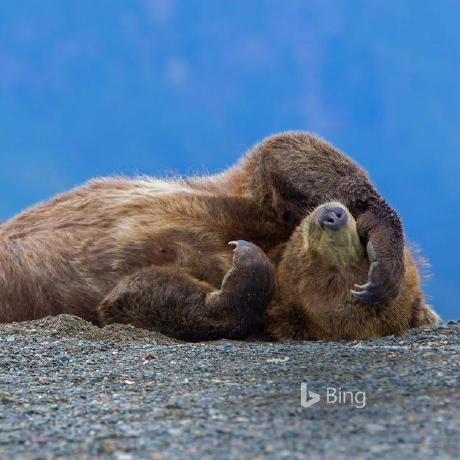
\includegraphics[scale=0.0574]{./PageDesign/YourPic.jpg}}; % add YourPic.jpg in the upper directory "PageDesign"
	\end{tikzpicture}
\end{textblock*}
\begin{textblock*}{21cm}(16.3cm,25cm)	
	
\end{textblock*}
\vspace*{10.5em} 		
	\section{Arbeitserfahrungen}
	
\cventrynocomma{}{*Wissenschaftlicher Mitarbeiter}{\hfill \normalfont \underline{11/2016 - 10/2019}}{Institut für Baumechanik und Numerische Mechanik, Uni Hannover, Deutschland}{}{
	\textbf{$\bullet$\hspace{0.63em}Schädigung- und Werkstoffmechanik, Stochastische Zuverlässigkeitsanalyse}
	%, \textbf{Numerische mechanics}	
	\begin{itemize}%
		%\item[\textit{Tasks}:] %\begin{itemize} DFG founded international training project
		\item Stochastische Materialmodellierung durch Zufallsprozess.
		%\item Zuverlässigkeitsschätzung von Werkstoffstrukturen mittels Monte-Carlo-Simulation.  %stochastische Prozess  
		\item Vorhersage der Sicherheit und Lebensdauer von Bauteilen. 
		%
		%	(z.B. 3Mon. gedauert Experiment wird innerhalb 10Min. simuliert.)  
			%\item Monte-Carlo simulation of stochastic process for structure reliability assessment.
			%\item High performance  non-linear FE analysis for high-cycle fatigue (one million cycles in minutes).
			%\item Large scale data visualisation.
%			\item  with life-cycle prediction.
%		\end{itemize} 
 	\end{itemize}
 	\textbf{$\bullet$\hspace{0.63em}Koordination wissenschaftlicher Veranstaltungen, Betreuung von Studierenden}
 	\begin{itemize}
 		\item Als Koordinator zuständig für Institut-Seminar (2017) und Winter-School (2018). 
 		\item Betreute zwei Bachelorarbeiten und eine Masterarbeit.
 	\end{itemize}
}
 
  \cventrynocomma{}{Gastforscher}{\hfill\normalfont {\underline{01/2019 - 07/2019}}}{Laboratoire de Mécanique et Technologie, Universit\'e Paris-Saclay, Frankreich}{}{
 	\textbf{$\bullet$\hspace{0.63em}Algorithmenentwicklung, Daten-Analyse} 
 	\begin{itemize}
 			\item Finite-Elemente-Berechnung der Ermüdungsschädigung. 
 		%\item  Optische Messung von mechanischer Verformung und Rissentwicklung im Betonträger.
 		%\item Parallelisierte Berechnung von lokalen FE-Moduls, Extrapolation von Zeitreihendaten. % Distributed computing, parallelisation of local FE module,  model extrapolation. 
 		\item Visualisierung, Statistik und Regressionsanalyse von Mess- und Berechnungsdaten.
 \end{itemize}}
 
\cventrynocomma{}{*Studentische Hilfskraft}{\hfill\normalfont \underline{03/2015 - 03/2016}}{Institut für  Wissenschaftliches Rechnen, TU Braunschweig, Deutschland}{}{
	\textit{\textbf{$\bullet$}}\hspace{0.63em}\textbf{Sensor-Fusion, Parameter-Identifikation} 
	\begin{itemize}%  
		\item Daten-Assimilation mittels 4D-Variation und Ensemble-Kalman-Filter (EnKF).
		\item Identifikation der Materialparameter und geometrischer Unsicherheit mit Sensordaten.
		%Referenzlösung erstellt mittels Open-Source-FEA-Software FEAP (entwickelt von UC Berkeley).%Geometrische Parameter-Identifikation aus einer Stahlplatte unter Spannung und Kompressionstest. Das Ziel war um die Position und Größe einer kreisförmigen Aufnahme in einer Stahlplatte zu identifizieren. Der Stand und Messdaten wurden auf der Open-Source Finite-Elemente Software FEAP (UC Berkeley) simuliert, doch der Posterior wurde durch EnKF identifiziert.  %For the simulation is used the ensemble Kalman filter and FE software FEAP (UC Berkeley).
\end{itemize}}

\cventrynocomma{}{Prozess Ingenieur~}{\small -Yutong Bus, Zhengzhou, China \normalsize \hfill\normalfont \underline{06/2013 - 09/2013}}{}{}{\begin{itemize}%
		\item 
		Statistische Qualitätskontrolle  der Elektrophorese-Behandlungsprozessen.
\end{itemize}}
\cventrynocomma{}{Qualitätsingenieur-Oberfläche~}{\small -\textit{Praktikum}, Xi'an Aero-Engine, Xi'an, China\hfill\normalsize \underline{06/2012 - 07/2012}}{}{}{\begin{itemize}%
		\item Oberflächeninspektion und Qualitätskontrolle der
		Triebwerksblätter mittels CMM.
\end{itemize}}
\cventrynocomma{}{Computertechniker~}{\small -\textit{Teilzeit}, Hasee Computer, Zhengzhou, China \normalsize \hfill  \underline{01/2011 - 06/2013}}{}{}{
	\begin{itemize}%
		\item Os- und Hardwarewartung, Aufbauen von Sicherheitssystemen.
	\end{itemize}
}
%\cventry{\normalfont \underline{07/2009 - 06/2013}}{IT-Administrator}{Teilzeit}{Yuke Technology}{Zhengzhou, China}{
%	\begin{itemize}%
%		\item Systemwartung Linux-Server.
%\end{itemize}}
\section{Ausbildungen}
\cventry{\normalfont \underline{11/2016 - 11/2020}}{\textbf{Promotion in Numerischer Mechanik}}{Note: {sehr gut}}{\newline  Leibniz Universität Hannover, Deutschland}{}{
\begin{itemize}%	
	\item[$\bullet$] \textit{Dissertation: {Stochastishe Modellierung und Numerische Simulation von Ermüdungsschädigung.}}
	\item Finite-Elemente-Analyse (FEA), Paralleles Rechnen.
	\item Werkstoffmechanik, stochastischer Prozess.
	%	\item Im Vergleich mit klassischen Monte-Carlo, bezüglich die Berechnungskosten.
\end{itemize}
}
\cventry{\normalfont \underline{10/2013 - 05/2016}}{M.Sc. \textbf{Computational Sciences in Engineering (CSE)}}{Note: 2,1}{}{\newline Technische Universität Braunschweig, Deutschland}{
	\begin{itemize}
		\item Bayessche Statistik, Festkörper- und Strömungsmechanik.
		\item Numerische Verfahren für Differenzialgleichungen, Linear- und Nichtlineare Systemen. 
		%	\item Masterarbeit \textit{Note:\textbf{1,3}}, Projektarbeit \textit{Note:\textbf{1,0}}.
		%	\hspace{-1em}*\hspace{1em}  \item gute Kenntnisse in Datenanalyse und Verarbeitung.
\end{itemize}} 
%\begin{textblock*}{2cm}(2cm,22.5cm)
%	*  
%\end{textblock*}
\footnotetext{* Arbeitszeugnisse wurden beigefügt.} 
%\footnotetext{* Dissertation wurde am 16.06.2020 abgegeben.}
%\hspace*{-0.4cm}
% arguments 3 to 6 can be left empty
\cventry{\normalfont \underline{09/2009 - 06/2013}}{B.Ing. \textbf{Qualität- und Zuverlässigkeit-Ingenieurwissen}}{GPA: 83/100}{}{\newline Zhengzhou University of Aeronautics, China}{\begin{itemize}
		\item Total-Quality-Management (TQM), Qualitätsoptimierung.
		%	\item  Total-Quality-Management (TQM).
		\item Toolkit zur Zuverlässigkeitsanalyse.  
		%		\item , ERP.
\end{itemize}}
%\newpage
%\vspace{-2em}
\section{Studien- und Abschlussarbeiten}
%\hspace*{-0.4cm}
\cventry{\normalfont \underline{10/2015 - 04/2016}}{*Masterarbeit}{Note: {1,3}}{}{TU Braunschweig}{
	\textit{\textbf{$\bullet$}}\hspace{0.63em}\textbf{Unsicherheitsquantifizierung} des Schadens im Betonträger durch Multi-Level-Monte-Carlo-Verfahren
	\begin{itemize}%
		\item Schädigungsmodellierung von Stahlbeton.
		\item Modellierung unsicherer Materialeigenschaften mittels Zufallsfelder.
	%	\item Im Vergleich mit klassischen Monte-Carlo, bezüglich die Berechnungskosten.
\end{itemize}} 
\footnotetext{* Demonstriert im beigefügten Portfolio (in englischer Sprache).}
\cventry{\normalfont \underline{11/2014 - 05/2015}}{*Projektarbeit} {Note: {1,0}}{}{TU Braunschweig}{
	\textit{\textbf{$\bullet$}}\hspace{0.63em}\textbf{Datenassimilation} durch Ensemble Kalman Filter und 4D Variationsmethode
	\begin{itemize}%
		\item Vergleich der Effizienz und Genauigkeit beider Methoden.
		\item  Lösen mehrdimensionales chaotisches System durch 4-stufigen Runge-Kutta Verfahren.
\end{itemize}}
\cventry{\normalfont \underline{12/2012 - 05/2013}}{Bachelorarbeit}{Note: {sehr gut}}{Zhengzhou University of Aeronautics}{}{\textit{\textbf{$\bullet$}}\hspace{0.63em}\textbf{Qualitätsoptimierung} von Bankdienstleistungen aus technischer Perspekt.
	\begin{itemize}%
		\item Hauptkomponentenanalyse des multivariaten Bewertungsmodells der Servicequalität.
		\item Topologiebasierte Service-Netzwerk-Optimierung.
		\item  Ergonomische Verbesserung der Zugänglichkeit von Geldautomaten.
\end{itemize}}


	\section{Weitere Fähigkeiten und Interessen}
\cvitem{Software}{Matlab, Abaqus (mit Python-script), SPSS.}{}{}
\cvitem{Coding}{C++ (QT, Python-test), Python (Pandas, Scipy, TensorFlow).}
%							\cvitem{\hspace{-1cm}Programming}{Matlab, Python}{}{}
\cvitem{Sprachen}{Deutsch (fließend), English (fließend), Mandarin (Muttersprache).}{}{}
%	\cvitem{Sprachen}{English (Arbeitssprache), Chinese (Muttersprache), French \& Portugiese (Grundkenntnisse) }{}{}
%		\cvitem{}{\hspace{5.2em}EU/China Führerschein vorhanden (ohne Verkehrsverstöße seit 5 Jahren)}{}{}
%\cvitem{Licenses}{EU and chinese driving license}{}{}
\cvitem{Hobbys}{Sportfishing, Saxophon, Fotografieren.}{}{}
%\hspace{-2em}*\hspace{2em} 
%, EU and Chinese driving license
%\begin{textblock*}{2cm}(2cm,18.1cm)
%*  
%\end{textblock*}
% arguments 3 to 6 can be left empty

\section{Vorträge bei internationalen akademischen Veranstaltungen}
%\cventry{\normalfont (Dez. 2017)}{Senlis, Frankreich}{}{7th International Conference Fatigue Design}{}{}
\cventry{\normalfont \underline{05/2018}}{Poitier, Frankreich}{}{12th International Fatigue Congress}{}{\textit{Vortrag: On the time discritisation effect of stochastic damage evolution.}}
\cventry{\normalfont \underline{06/2019}}{Crete, Griechenland}{}{3rd International Conference on Uncertainty Quantification \newline in Computational Sciences and Engineering}{}{\textit{Vortrag: Stochastic modelling of fatigue process.}}
\cventry{\normalfont \underline{09/2019}}{Barcelona, Spanien}{}{15th International Conference on Computational Plasticity}{}{\textit{Vortrag: Modelling approach and efficient numerical scheme for stochastic fatigue process.}}
\section{Veröffentlichung}
Stochastic Material Modeling for Fatigue Damage Analysis. \textit{W.Zhang, A.Fau, U.Nackenhorst, R.Desmorat}\newline In: Virtual Design and Validation. Springer, Cham, 2020. S. 329-347. [In englischer Sprache] 
							
								\section{Auszeichnungen}
								\cventry{\normalfont \underline{11/2013}}{CSE "Junior"-Stipendium}{}{}{}{Technische Universität Braunschweig. Braunschweig, Deutschland}
								\cventry{\normalfont \underline{06/2013}}{		"Ausgezeichneter Absolvent"}{}{}{}{Zhengzhou University of Aeronautics. Zhengzhou, China}
								\cventry{\normalfont \underline{10/2012}}{Stipendium Jahr 2012}{}{}{}{Zhengzhou University of Aeronautics. Zhengzhou, China}
								\cventry{\normalfont \underline{09/2011}}{1. Platz bei studentischem Karriereplanwettbewerb}{}{}{}{Zhengzhou University of Aeronautics. Zhengzhou, China}
								\cventry{\normalfont \underline{06/2011}}{2. Platz bei studentischem Musikwettbewerb der Provinz Henan}{}{}{}{Musician Association of Henan Province, Zhengzhou, China}
								\clearpage

%\newpage
\setlength{\parskip}{0.25em}
\renewcommand*{\thefootnote}{\fnsymbol{footnote}}
\setcounter{footnote}{0}
%\makecvtitle

\begin{textblock*}{21cm}(0cm,-0.08cm)	
	\includegraphics[scale=1]{./PageDesign/title.eps}
\end{textblock*}

\begin{textblock*}{21cm}(2cm,1.7cm)	
	\Huge \textcolor{white}{Weiran Zhang}
\end{textblock*}

\begin{textblock*}{21cm}(2cm,3.4cm)	
	\Large \textbf{Development, Simulation}
	%	\large{\textbf{Key Skills}}: Stochastic Modelling, Computational Mechanics \normalsize	
\end{textblock*}
\begin{textblock*}{21cm}(2cm,4.3cm)	
	%	Anschrift: Richterstr. 19 | 38106 Braunschweig | Deutschland\\
	\faXing~ \href{https://www.xing.com/profile/Weiran_Zhang4/cv}{Xing} ~ \faLinkedinSquare~ \href{https://www.linkedin.com/in/weiran-zh/}{Linkedin} ~ \faGlobe~\href{http://www.weiran.de}{weiran.de}\\
	\faEdit\hspace{0.45em}\href{mailto:weiran-zhang@outlook.com}{weiran-zhang@outlook.com} \\
	\faPhoneSquare~ +49~(0)176-2136 5452
	%Age: 25 | Civil status: Single | Nationality: Chinese
\end{textblock*}
\begin{textblock*}{21cm}(15cm,1.2cm)	
	%\includegraphics[scale=0.055]{picture2}
	%\noindent\shadowimage[scale=0.055]{picture2}\par\bigskip
	\begin{tikzpicture}[overlay]
	\node[opacity=1] at (2.2,-2.7)%%2.5,-2.3
	{\includegraphics[scale=0.0574]{../../signature/potrait-s_Zhang.jpg}};
	\end{tikzpicture}
\end{textblock*}
\begin{textblock*}{21cm}(16.3cm,25cm)	
	%\includegraphics[scale=0.055]{picture2}
	%\noindent\shadowimage[scale=0.055]{picture2}\par\bigskip
	\begin{tikzpicture}
	%\node[opacity=0.1] {\includegraphics[scale=1]{Bosch.eps}};
	\end{tikzpicture}
\end{textblock*}
\vspace*{9em} 	
	\section{Working Experiences}
\cventry{\normalfont (Nov 2016- Oct 2019)}{Research Assistant}{}{Institute of Mechanics and Computational Mechanics}{Leibniz University Hannover, Germany}{
	\textit{\textbf{*Topics:}}  \textbf{Stochastic reliability analysis}, \textbf{Computational mechanics}
	\begin{itemize}%
		%\item[\textit{Tasks}:] %\begin{itemize} DFG founded international training project
			\item Monte-Carlo simulation of stochastic process for structure reliability assessment.
			\item High performance  non-linear FE analysis for high-cycle fatigue (one million cycles in minutes).
			%\item Large scale data visualisation.
%			\item  with life-cycle prediction.
%		\end{itemize} 
 	\end{itemize}}
 \cventry{\normalfont (2017- 2019 for 6 months) }{Research Exchange in EU}{}{LMT Cachan, \newline Universit\'e Paris-Saclay}{France}{
\textbf{\textit{Topics:} Data analysis, Optical measurement, Algorithm optimisation}  
\begin{itemize}
%	\item Infrared and visible-light measurement of temperature distribution and crack propagation.
	\item Optical measurement of material deformation and crack propagation.
	\item Visualisation, statistics and regression analysis of fatigue scatters.
\end{itemize}
}
\cventry{\normalfont (Mar 2015- Jul 2015)}{Research Assistant}{}{Institute of Scientific Computing}{\newline Technical University Braunschweig, Germany}{
\textbf{\textit{Topics:} Multi-sensor data fusion, Bayesian statistics}  	\begin{itemize}%
		\item Parameter identification with ensemble Kalman filter (EnKF).
		\item Data assimilation with 4D-Var and EnKF methods.
		%Reference solution with open-source FE software FEAPpv (from UC Berkeley).%Geometrische Parameter-Identifikation aus einer Stahlplatte unter Spannung und Kompressionstest. Das Ziel war um die Position und Größe einer kreisförmigen Aufnahme in einer Stahlplatte zu identifizieren. Der Stand und Messdaten wurden auf der Open-Source Finite-Elemente Software FEAP (UC Berkeley) simuliert, doch der Posterior wurde durch EnKF identifiziert.  %For the simulation is used the ensemble Kalman filter and FE software FEAP (UC Berkeley).
\end{itemize}}
\cventry{\normalfont (Jun 2013- Sept 2013)}{Process Engineer}{}{Yutong Bus}{Zhengzhou, China}{\begin{itemize}%
		\item Statistical quality control of electrophoresis treating process.
\end{itemize}}
\cventry{\normalfont (Jun 2012- Jul 2012)}{Surface Quality Engineer}{intern}{Xi'an Aero-Engine}{Xi'an, China}{\begin{itemize}%
		\item  Optical inspection of aero-engine blades with CMM.
\end{itemize}}


\cventry{\normalfont (Jul 2009- Jun 2013)}{IT Administrator}{part-time}{Yuke Technology}{Zhengyang, China}{
	\begin{itemize}%
			\item Linux server maintenance,  LAN construction and client control. 
\end{itemize}}
\cventry{\normalfont (Jan 2011- Jun 2013)}{Hardware Technician}{part-time}{Hasee Computer}{Zhengzhou, China}{
	\begin{itemize}%
		\item Hardware maintenance and data recovery, construction of safety system.
	\end{itemize}
}
\footnotetext{* Demonstrated by the attached portfolio.}
\section{University Projects}
%\hspace*{-0.4cm}
\cventry{\normalfont (Oct 2015- Apr 2016)}{*Master Thesis}{German Note: \textbf{1,3}}{}{TU Braunschweig}{
	\textit{\textbf{Topic}}: \textbf{Uncertainty Quantification} of damage in RC beam using multilevel Monte-Carlo method
	\begin{itemize}%
		\item Elasto-damage reinforced concrete model with perfect bounding hypothesis,
		\item Modelling of uncertain material properties using random field and spectral approximation,
		\item Application and comparison of multilevel and classical Monte-Carlo methods in efficiency and accuracy.
\end{itemize}} 
%\footnotetext{* see attached portfolio for demonstration.}
\cventry{\normalfont (Nov 2014- May 2015)}{*Project Thesis} {German Note: \textbf{1,0}}{}{TU Braunschweig}{
	\textit{\textbf{Topic}}: \textbf{Data assimilation} with ensemble Kalman filter and four-dimensional variation method
	\begin{itemize}%
		\item Comparison on the efficiency and accuracy of the 4D-Var and EnKF methods.
		\item 4th order Runge-Kutta solution of multi-dimensional chaotic system.
\end{itemize}}
\cventry{\normalfont (Dec 2012- May 2013)}{Bachelor Project}{record: \textbf{excellent}}{Zhengzhou University of Aeronautics}{}{\textit{\textbf{Topic}}: \textbf{Quality optimisation} of banking service in less-developed region
	\begin{itemize}%
		\item Principal component analysis of service quality rating model.
		\item Topologie based service network optimisation.
		\item  Ergonomie improvement of ATM accessibility.
\end{itemize}}

\newpage
\footnotetext{* Two reference letters from former employers attached.} 
\section{Academic Education}
\cventry{\normalfont (Nov 2016- Sept 2020)}{\textbf{Promotion in Computational Mechanics}}{\textit{Defence date: 11.11.2020}}{\newline Leibniz University Hannover, Germany}{}{\textbf{\textit{Dissertation:}} Stochastic Modelling and Numerical Simulation of fatigue damage.}
\cventry{\normalfont (Oct 2013- May 2016)}{*M.Sc.}{}{\textbf{Computational Sciences in Engineering (CSE)}}{\newline Technical University Braunschweig, Germany}{
	\begin{itemize}
		\item Applied mathematics, mechanics and statistics.
				\item  Modelling and scientific computing.
		\item Master thesis and project thesis in excellent record.
\end{itemize}} 
%*~M.Sc.%\footnotetext{* two reference letters from research institute and company are attached below.}
\cventry{\normalfont (Sept 2009- Jun 2013)}{B.Eng.}{}{\textbf{Quality and Reliability Engineering}}{\newline Zhengzhou University of Aeronautics, China}{\begin{itemize}
		\item ISO 9000/14000 standards.
		\item Total quality management (TQM).
		\item Toolkit for reliability assessment, statistical process control. 
\end{itemize}}
\section{Further Skills and Interests}
\cvitem{Coding}{Matlab, C++ (Python test, QT), Abaqus (manipulated by Python script)}{}{}
%							\cvitem{\hspace{-1cm}Programming}{Matlab, Python}{}{}
\cvitem{Language}{English (fluent), German (fluent), Mandarin (native)}{}{}
%\cvitem{Language}{German (working language), Chinese (native), French \& Portugiese (entry level) }{}{}
%	\cvitem{}{\hspace{5.4em}EU and Chinese driving license available (without any fines/penalty in the past 5 years)}{}{}
%\cvitem{Licenses}{EU and chinese driving license}{}{}
\cvitem{Hobbies}{Sport fishing, Saxophone.}{}{}
%\hspace{-2em}*\hspace{2em} 
%, EU and Chinese driving license
%\begin{textblock*}{2cm}(2cm,18.1cm)
%*  
%\end{textblock*}

\section{Presentation at International Academic Events}

\cventry{\normalfont (May 2018)}{Poitier, France}{}{12th International Fatigue Congress}{}{\textit{Presentation: On the time discritisation effect of stochastic damage evolution.}}
\cventry{\normalfont (Jun 2019)}{Crete, Greece}{}{3rd International Conference on Uncertainty Quantification in Computational Sciences and Engineering}{}{\textit{Presentation: Stochastic modelling of fatigue process.}}
\cventry{\normalfont (Sept 2019)}{Barcelona, Spain}{}{15th International Conference on Computational Plasticity}{}{\textit{Presentation: Modelling approach and efficient numerical scheme for stochastic fatigue process.}}
\section{Publication}
Stochastic Material Modelling for Fatigue Damage Analysis. In: Virtual Design and Validation. Springer, Cham, 2020. S. 329-347. 
  % arguments 3 to 6 can be left empty
														\section{Awards}
								\cventry{\normalfont (Nov 2013)}{CSE "Junior"-Scholarship}{}{}{}{Technical University Braunschweig. Braunschweig, Deutschland}
								\cventry{\normalfont (Jun 2013)}{Excellent Graduate}{}{}{}{Zhengzhou University of Aeronautics. Zhengzhou, China}
								\cventry{\normalfont (Oct 2012)}{University Scholarship}{}{}{}{Zhengzhou University of Aeronautics. Zhengzhou, China}
								\cventry{\normalfont (Sept 2011)}{First Place of Undergraduates Career Plan Competition}{}{}{}{Zhengzhou University of Aeronautics. Zhengzhou, China}
								\cventry{\normalfont (Jun 2011)}{Second Place of University Music Competition of Henan Province}{}{}{}{Musician Association of Henan Province, Zhengzhou, China}
								\clearpage
%
%\includepdf[page={1},addtotoc={1,section,1,Arbeitzeugnis Prof. Nackenhorst,mylabel}]{../../recommendation/Arbeitszeugnis_IBNM_Zhang_2020.pdf}
%\includepdf[page={1},addtotoc={
%	1,section,2,Arbeitzeugnis Prof. Jacob,mylabel}]{../../recommendation/Ref_Jacob.pdf}
%\includepdf[page={1-2},addtotoc={
%	1,section,3,Arbeitzeugnis Prof. Matthies,mylabel}]{../../recommendation/recommendation_Zhang_final.pdf}
%\includepdf[page={1-6},addtotoc={
%	1,section,4,Portfolio,p1}]{../../Onesubsea/Portfolio.pdf}
%\includepdf[page={1-3},addtotoc={
%	1,section,5,Masterabschluss,mylabel}]{../../Urkunde/MasterUrkunde.pdf}
%%\includepdf[page={1-2}]{../../Urkunde/MasterUrkunde.pdf}
%\includepdf[page={1},addtotoc={
%	1,section,6,Anerkennung Bachelorabschluss,mylabel}]{../../Urkunde/APS.pdf}
%
%\includepdf[page={1},addtotoc={
%	1,section,7,Bachelorabschluss,mylabel}]{../../Urkunde/BachelorUrkundeQue.pdf}
\end{document}


%% end of file `template.tex'.
